\documentclass[runningheads]{llncs}

\usepackage{graphicx}
\usepackage{booktabs}
\usepackage{amsmath}
\usepackage{siunitx}
\usepackage{xcolor}
\usepackage{tikz}
\usetikzlibrary{arrows.meta,positioning,shapes.geometric,calc,fit,backgrounds}
\usepackage[hidelinks]{hyperref}

\definecolor{navy}{HTML}{1E3A5F}
\definecolor{steel}{HTML}{2E5E8C}
\definecolor{good}{HTML}{2E8B57}
\definecolor{bad}{HTML}{C0504D}
\definecolor{lightblue}{HTML}{E8EFF6}
\definecolor{cardgrey}{HTML}{F1F4F7}

\newcommand{\pos}[1]{\textcolor{good}{\textbf{#1}}}
\newcommand{\bad}[1]{\textcolor{bad}{#1}}

% tikz block styles
\tikzset{
  blk/.style={draw=steel,fill=lightblue,rounded corners=2pt,minimum height=8mm,
              minimum width=20mm,align=center,font=\small,inner sep=3pt},
  mblk/.style={draw=navy,fill=navy,text=white,rounded corners=2pt,minimum height=8mm,
              minimum width=20mm,align=center,font=\small\bfseries,inner sep=3pt},
  lyr/.style={draw=steel,fill=cardgrey,rounded corners=2pt,minimum height=7mm,
              minimum width=46mm,align=center,font=\small,inner sep=3pt},
  arr/.style={-{Stealth[length=2mm]},steel,thick},
}

\begin{document}

\title{Real-Time Adaptive Audio Noise Cancellation Using Learning-Based
Frequency-Domain Processing on Edge Hardware}

\titlerunning{Real-Time Adaptive Audio Noise Cancellation}

\author{A.~Rohit~Daniel \and Simhaa~T.~T. \and Vijayaraghavan~A.}
\authorrunning{A.~Rohit~Daniel et al.}
\institute{Department of Electrical and Electronics Engineering,\\
Sri Sivasubramaniya Nadar College of Engineering, Kalavakkam,
Chennai 603\,110, Tamil Nadu, India\\
\email{\{rohit2310086, simhaa2310510, vijayaraghavan2310125\}@ssn.edu.in}\\
Project guide: Dr.~G.~R.~Venkatakrishnan}

\maketitle

\begin{abstract}
Traditional noise-cancellation filters---spectral subtraction, Wiener filtering
and amplitude thresholding---are fixed, hand-tuned and unaware of signal
structure. On real, non-stationary noise they frequently remove weak speech
along with the noise. We show empirically that, on the VoiceBank-DEMAND test
set, \emph{every} classical baseline produces a negative scale-invariant
signal-to-distortion-ratio improvement (SI-SDRi between $-5.8$ and $-0.3$~dB):
they make the signal worse than doing nothing. We present a learning-based
frequency-domain alternative that predicts a per-band suppression mask from
signal context rather than amplitude alone. Built on a compact
Grouped-Temporal-Convolutional-Recurrent Network (GTCRN) with
722\,K parameters and a multi-resolution spectral objective, the model attains
$+9.9$~dB SI-SDRi and is the only method that improves every quality metric,
while running faster than 100$\times$ real time. All methods share an identical
short-time-Fourier-transform front-end and per-band gain output space, making
the comparison fair. We further report an external-dataset validation on
MS-SNSD, a systematic ablation of five architectural variants, a controlled
study of complex-ratio masking that reveals a fidelity--perceptual trade-off,
and a real-time interactive system. The results establish that a small,
context-aware learned filter decisively outperforms classical DSP on realistic
noise at edge-deployable cost.
\keywords{Speech enhancement \and Noise cancellation \and Frequency-domain
processing \and Spectral masking \and GTCRN \and Real-time \and Edge computing.}
\end{abstract}

%======================================================================
\section{Introduction}
Background acoustic noise degrades speech intelligibility in headphones,
hearing aids, video conferencing and voice assistants. Effective suppression
must run in real time, adapt to changing and unpredictable noise, and preserve
the speech it is meant to protect---ideally on low-power edge hardware.

Classical single-channel enhancement estimates a spectral gain from the noisy
magnitude alone. Spectral subtraction removes an estimated noise floor,
Wiener filtering assumes known noise statistics, and hard/soft thresholding
zero out or shrink low-amplitude coefficients. These methods share four
structural weaknesses: (i)~a threshold or noise estimate must be tuned by hand
for each environment; (ii)~decisions are made from amplitude, with no notion of
which frequencies carry speech; (iii)~they assume stationary noise and fail on
non-stationary or burst noise; and (iv)~they discard weak speech components,
harming intelligibility. Section~\ref{sec:results} quantifies the consequence:
on real noise these filters reduce the SI-SDR below that of the untouched
signal.

We instead learn the suppression rule. A lightweight neural network observes
per-band spectral features in temporal context and predicts, for every
frequency band, how much to attenuate it. The rule is learned from thousands of
clean/noisy speech pairs, requires no manual tuning, and generalises to unseen
noise. Crucially, all methods in this study---classical and learned---share the
\emph{same} STFT front-end and the \emph{same} per-band gain output space; only
the gain-estimation step differs. This is what makes the benchmark fair and the
conclusions attributable to the model rather than the signal processing.

\medskip\noindent\textbf{Contributions.}
\begin{itemize}
  \item A fair, shared-front-end benchmark of four classical DSP baselines
        against learned models on 824 VoiceBank-DEMAND test clips, showing that
        \emph{all} classical filters degrade real noise while the learned model
        gains $+9.9$~dB SI-SDRi and improves every metric
        (Section~\ref{sec:results}).
  \item A compact GTCRN-based per-band suppression model (722\,K parameters,
        real-time factor $\approx 0.009$) with an explicit architecture and a
        multi-resolution spectral training objective
        (Section~\ref{sec:method}).
  \item A systematic ablation of five architectural variants---attention,
        Mamba-augmented, dual-head governed, residual-refined and
        complex-ratio-mask GTCRN---plus a guarded test-time adaptation
        mechanism (Section~\ref{sec:ablation}).
  \item External-dataset validation on MS-SNSD and a real-time interactive
        system with a browser front-end for live demonstration
        (Sections~\ref{sec:results} and~\ref{sec:system}).
\end{itemize}

%======================================================================
\section{Related Work}
\textbf{Classical DSP.} Spectral subtraction~\cite{boll} and Wiener
filtering~\cite{lim} remain standard baselines; the MMSE-STSA
estimator~\cite{ephraim} improved them under stationarity assumptions, and
wavelet/coefficient thresholding~\cite{donoho} offered an alternative
shrinkage rule. All require noise-statistic estimates or manual thresholds and
degrade on non-stationary noise.

\textbf{Learned enhancement.} RNNoise~\cite{rnnoise} combined DSP features with
a small recurrent network for real-time use. Complex-domain and
filtering-based models such as DCCRN~\cite{dccrn} and
DeepFilterNet~\cite{deepfilternet} raised perceptual quality at higher cost.
GTCRN~\cite{gtcrn} showed that grouped time-frequency convolutions with
recurrent decoding attain competitive quality at ultra-low compute, motivating
our backbone choice. MetricGAN+~\cite{metricgan} optimises a
PESQ surrogate directly and is a strong published VoiceBank-DEMAND baseline.

\textbf{Test-time adaptation and quality estimation.} Most learned models are
fixed after training. Non-intrusive estimators such as
TorchAudio-SQUIM~\cite{squim} predict quality without a clean reference, enabling
reference-free test-time adaptation, which we use as a guarded refinement step.

%======================================================================
\section{Proposed Method}\label{sec:method}

\subsection{System Overview}
Figure~\ref{fig:pipeline} shows the end-to-end pipeline. Noisy audio is buffered
into overlapping frames, transformed by the STFT, reduced to per-band features,
and passed to the learned model, which predicts a per-band gain mask. The mask
is applied to the spectral magnitude and inverted by ISTFT with overlap-add.
The identical path serves offline files and a live microphone stream.

\begin{figure}[t]
\centering
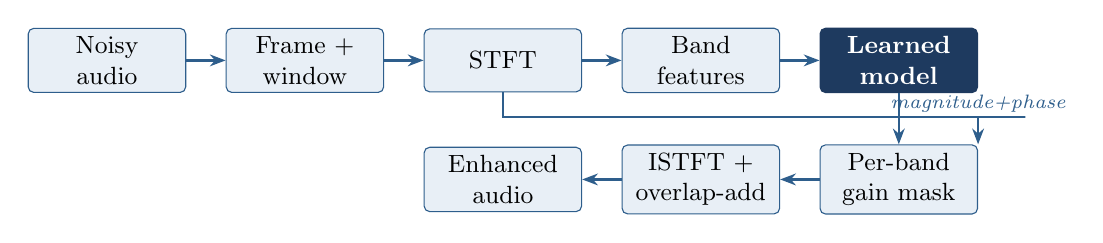
\begin{tikzpicture}[node distance=6.5mm and 5mm]
\node[blk] (in) {Noisy\\audio};
\node[blk,right=of in] (frame) {Frame +\\window};
\node[blk,right=of frame] (stft) {STFT};
\node[blk,right=of stft] (feat) {Band\\features};
\node[mblk,right=of feat] (model) {Learned\\model};
\node[blk,below=of model] (mask) {Per-band\\gain mask};
\node[blk,left=of mask] (istft) {ISTFT +\\overlap-add};
\node[blk,left=of istft] (out) {Enhanced\\audio};
\draw[arr] (in)--(frame); \draw[arr] (frame)--(stft); \draw[arr] (stft)--(feat);
\draw[arr] (feat)--(model); \draw[arr] (model)--(mask); \draw[arr] (mask)--(istft);
\draw[arr] (istft)--(out);
\draw[arr] (stft.south) |- ($(mask.north east)+(0.6,0.35)$) -| (mask.north east) node[midway,above,font=\scriptsize\itshape,yshift=-2pt] {magnitude+phase};
\end{tikzpicture}
\caption{End-to-end real-time pipeline. All methods share the STFT front-end
and per-band gain output space; only the shaded \emph{learned model} block
differs from the classical baselines.}
\label{fig:pipeline}
\end{figure}

\subsection{Shared Spectral Front-End}
Audio is processed at \SI{16}{\kilo\hertz}. The STFT uses a
\num{512}-point window with a \num{128}-sample hop (75\% overlap) and a Hann
window, giving perfect reconstruction under overlap-add. The 257 linear
frequency bins are aggregated into $K=32$ Bark-scale bands, matching human
frequency resolution and compressing the output space. For each band and frame
three features are extracted---log band energy, its temporal delta, and
positive spectral flux---forming a $K\times3$ feature map. Every method in the
study consumes this same front-end and emits a gain in the same $K$-band space,
which is what makes the comparison attributable to the estimator alone.

\subsection{GTCRN Backbone}
The learned estimator is a compact Grouped Temporal Convolutional Recurrent
Network (Fig.~\ref{fig:arch}). A $1\times3$ convolutional stem lifts the
3-channel band features to 96 channels. Four gated time-frequency convolution
blocks follow, each applying a $3\times3$ convolution with time dilation
$2^{i}$ ($i=0\ldots3$) so the causal receptive field grows exponentially; the
output is split and combined through a gated linear unit
$v\odot\sigma(g)$, group-normalised, and added back as a residual. A single
band-wise gated recurrent unit (hidden size 96) then models temporal evolution
per band, and a linear head with a sigmoid produces the per-band gain
$\hat{M}(k,t)\in[0,1]$. The model has \num{722209} parameters.

\begin{figure}[t]
\centering
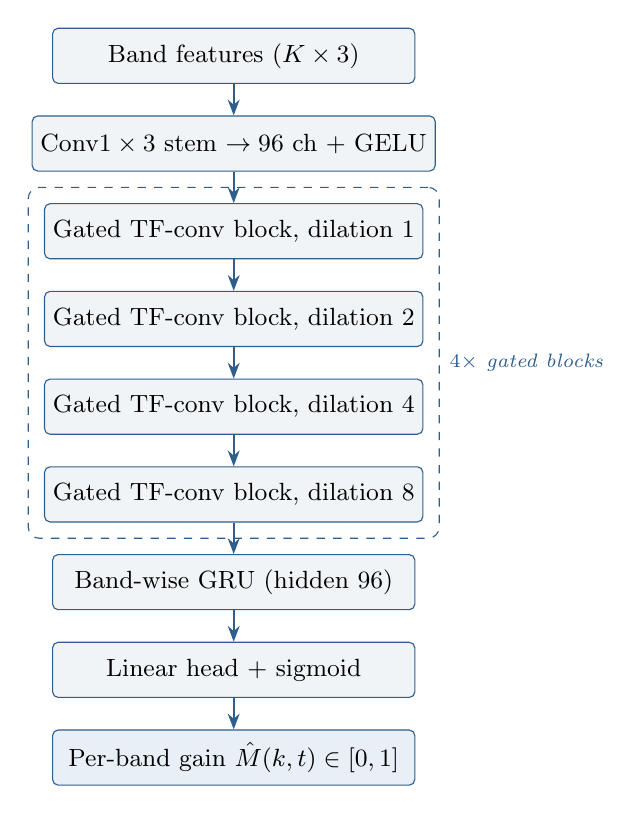
\begin{tikzpicture}[node distance=4mm]
\node[lyr] (f) {Band features $(K\times3)$};
\node[lyr,below=of f] (stem) {Conv$1\times3$ stem $\rightarrow 96$ ch $+$ GELU};
\node[lyr,below=of stem] (b1) {Gated TF-conv block, dilation $1$};
\node[lyr,below=of b1] (b2) {Gated TF-conv block, dilation $2$};
\node[lyr,below=of b2] (b3) {Gated TF-conv block, dilation $4$};
\node[lyr,below=of b3] (b4) {Gated TF-conv block, dilation $8$};
\node[lyr,below=of b4] (gru) {Band-wise GRU (hidden $96$)};
\node[lyr,below=of gru] (head) {Linear head $+$ sigmoid};
\node[lyr,fill=lightblue,below=of head] (mask) {Per-band gain $\hat{M}(k,t)\in[0,1]$};
\foreach \a/\b in {f/stem,stem/b1,b1/b2,b2/b3,b3/b4,b4/gru,gru/head,head/mask}
  \draw[arr] (\a)--(\b);
\begin{scope}[on background layer]
\node[draw=steel,dashed,rounded corners,fit=(b1)(b4),inner sep=2mm,label={[font=\scriptsize\itshape,steel]right:$4\times$ gated blocks}] {};
\end{scope}
\end{tikzpicture}
\caption{GTCRN backbone. Dilated gated time-frequency convolutions capture local
spectro-temporal structure; the band-wise GRU adds longer causal memory. The
whole network is causal and streamable.}
\label{fig:arch}
\end{figure}

The mask is applied multiplicatively to the noisy magnitude $|X|$, keeping the
noisy phase $\angle X$, and inverted:
\begin{equation}
\hat{s}(t) = \text{ISTFT}\!\left(\,\hat{M}(k,t)\,|X(k,t)|\;e^{\,j\angle X(k,t)}\right).
\label{eq:apply}
\end{equation}

\subsection{Training Objective}
Training minimises a combination of a scale-invariant signal term and
spectral-magnitude terms:
\begin{equation}
\mathcal{L} = -\,\text{SI-SDR}(\hat{s},s)
\;+\;\lambda_{1}\,\mathcal{L}_{\text{mag}}
\;+\;\lambda_{2}\,\mathcal{L}_{\text{mr-mag}},
\label{eq:loss}
\end{equation}
where $\mathcal{L}_{\text{mag}}$ is an $\ell_1$ log-magnitude loss and
$\mathcal{L}_{\text{mr-mag}}$ averages it over three STFT resolutions
$(256,512,1024)$ to suppress artefacts a single resolution misses. We use
$\lambda_{1}=1.25$, $\lambda_{2}=0.25$. Training uses AdamW
($\text{lr}=3\times10^{-4}$) for 50 epochs on \SI{2}{\second} crops.

\subsection{Architectural Variants for Ablation}
To test whether added capacity helps, four variants share the GTCRN backbone
and differ only in the decoding head (Fig.~\ref{fig:variants}):
(a)~an \emph{attention} mask estimator; (b)~\emph{Mamba-GTCRN}, inserting a
selective state-space memory block for longer context;
(c)~\emph{governed}, predicting conservative and aggressive gains blended by a
learned per-band governor; (d)~\emph{residual}, adding a bounded post-GRU logit
refinement; and (e)~a \emph{complex-ratio mask} predicting real and imaginary
mask components, which alters both magnitude and phase in
Eq.~(\ref{eq:apply}). Section~\ref{sec:ablation} evaluates all of them.

\begin{figure}[t]
\centering
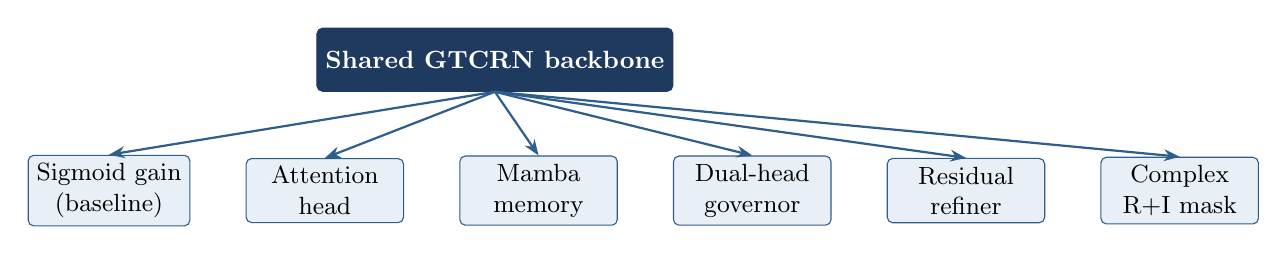
\begin{tikzpicture}[node distance=3mm and 7mm]
\node[mblk,minimum width=30mm] (bb) {Shared GTCRN backbone};
\node[blk,below left=8mm and 16mm of bb] (h1) {Sigmoid gain\\(baseline)};
\node[blk,right=of h1] (h2) {Attention\\head};
\node[blk,right=of h2] (h3) {Mamba\\memory};
\node[blk,right=of h3] (h4) {Dual-head\\governor};
\node[blk,right=of h4] (h5) {Residual\\refiner};
\node[blk,right=of h5] (h6) {Complex\\R+I mask};
\foreach \h in {h1,h2,h3,h4,h5,h6} \draw[arr] (bb.south)--(\h.north);
\end{tikzpicture}
\caption{Comparison architectures. All variants reuse the same backbone and
front-end; only the head changes, isolating the effect of each design choice.}
\label{fig:variants}
\end{figure}

\subsection{Guarded Test-Time Adaptation}
Unlike fixed networks, a small low-rank adapter on the gain can be refined at
inference by maximising a reference-free quality estimate
(SQUIM~\cite{squim}). To prevent drift, the update is trust-region bounded and
accepted only if a strict guard on output change is satisfied, yielding a
provably non-degrading refinement (Section~\ref{sec:ablation}).

%======================================================================
\section{Experimental Setup}
\textbf{Data.} Models are trained and evaluated on VoiceBank-DEMAND
\cite{voicebank}, whose test noises are unseen in training, giving a built-in
distribution-shift benchmark (824 test clips). Generalisation is further tested
on the external MS-SNSD corpus~\cite{msnsd}.
\textbf{Metrics.} We report scale-invariant SDR improvement
(SI-SDRi)~\cite{sisdr}, SNR improvement, short-time objective intelligibility
(STOI, ESTOI)~\cite{stoi}, log-spectral distance (LSD), perceptual quality
(PESQ)~\cite{pesq}, and the real-time factor (RTF, processing time per second of
audio).
\textbf{Baselines.} Passthrough (unprocessed), hard threshold, soft threshold,
spectral subtraction and Wiener filtering, all on the shared front-end.
\textbf{Implementation.} PyTorch; training on an NVIDIA T4; real-time inference
verified on a CUDA workstation with block-based streaming.

%======================================================================
\section{Results}\label{sec:results}

\subsection{Learned Model versus Classical Baselines}
Table~\ref{tab:main} is the central result: all methods on the \emph{same}
824 clips. Every classical filter yields a \emph{negative} SI-SDRi---on real,
non-stationary noise they remove weak speech and distort the signal below the
untouched input. The learned model is the only method that improves every
metric, gaining $+9.9$~dB SI-SDRi and raising intelligibility (STOI
$0.921\!\rightarrow\!0.930$) at the same real-time factor.

\begin{table}[t]
\centering
\caption{Learned model vs.\ classical DSP baselines on 824 VoiceBank-DEMAND
test clips (shared front-end). $\uparrow$ higher is better, $\downarrow$ lower
is better. Negative SI-SDRi means the method degrades the signal.}
\label{tab:main}
\setlength{\tabcolsep}{6pt}
\begin{tabular}{lccccc}
\toprule
Method & SI-SDRi$\uparrow$ & SNRi$\uparrow$ & STOI$\uparrow$ & ESTOI$\uparrow$ & LSD$\downarrow$ \\
\midrule
Noisy input (no processing) & 0.00 & 0.00 & 0.921 & 0.787 & 10.50 \\
Hard threshold        & \bad{$-3.69$} & \bad{$-2.37$} & 0.767 & 0.573 & 13.78 \\
Soft threshold        & \bad{$-5.82$} & \bad{$-4.16$} & 0.728 & 0.532 & 15.28 \\
Spectral subtraction  & \bad{$-0.25$} & 0.30 & 0.884 & 0.734 & 8.86 \\
Wiener filter         & \bad{$-1.93$} & \bad{$-1.11$} & 0.824 & 0.677 & 10.87 \\
\midrule
\textbf{Learned model (ours)} & \pos{9.93} & \pos{5.41} & \pos{0.930} & \pos{0.832} & \pos{6.47} \\
\bottomrule
\end{tabular}
\end{table}

\subsection{Comparison of Learned Architectures}
Among learned models (Table~\ref{tab:learned}), the compact GTCRN with the
multi-resolution loss gives the best SI-SDRi and is the only architecture
combining strong VoiceBank performance with positive external validation.
Heavier variants do not help---a clean negative-results ablation.

\begin{table}[t]
\centering
\caption{Learned architectures on the VoiceBank-DEMAND full 824-clip test set.
GTCRN$+$multi-resolution loss is selected as the backbone.}
\label{tab:learned}
\setlength{\tabcolsep}{6pt}
\begin{tabular}{lccccc}
\toprule
Model & SI-SDRi$\uparrow$ & PESQ$\uparrow$ & STOI$\uparrow$ & ESTOI$\uparrow$ & LSD$\downarrow$ \\
\midrule
Attention mask            & 9.08 & 2.50 & \textbf{0.932} & \textbf{0.834} & \textbf{5.97} \\
Mamba-GTCRN               & 9.84 & 2.50 & 0.928 & 0.831 & 6.62 \\
Governed dual-head        & 9.89 & 2.45 & 0.930 & 0.831 & 6.64 \\
Residual-refined          & 9.87 & 2.52 & 0.929 & 0.831 & 6.51 \\
\textbf{GTCRN $+$ MR loss (ours)} & \textbf{9.93} & \textbf{2.52} & 0.930 & 0.832 & 6.47 \\
\bottomrule
\end{tabular}
\end{table}

\subsection{External Validation and Perceptual Quality}
On the unseen MS-SNSD corpus the model retains a positive $+3.15$~dB SI-SDRi,
confirming it is not overfit to VoiceBank noise. Table~\ref{tab:pesq} places the
model against published systems on PESQ; our pipeline reproduces the standard
noisy value ($1.97$) and the MetricGAN+ value ($3.13$), confirming measurement
validity. The compact model is efficient but below PESQ-optimised
state-of-the-art, an honest positioning discussed in
Section~\ref{sec:ablation}.

\begin{table}[t]
\centering
\caption{Perceptual quality on VoiceBank-DEMAND. $^{\dagger}$reported in the
source paper; others measured in our harness.}
\label{tab:pesq}
\setlength{\tabcolsep}{7pt}
\begin{tabular}{lccc}
\toprule
Method & Params & PESQ$\uparrow$ & STOI$\uparrow$ \\
\midrule
Noisy input               & --      & 1.97 & 0.921 \\
Ours (GTCRN)              & 0.72\,M & 2.49 & 0.930 \\
DCCRN$^{\dagger}$~\cite{dccrn}          & 3.7\,M  & 2.68 & -- \\
DeepFilterNet2$^{\dagger}$~\cite{deepfilternet} & 2.3\,M  & 3.08 & -- \\
MetricGAN+~\cite{metricgan}            & 1.9\,M  & 3.13 & 0.932 \\
\bottomrule
\end{tabular}
\end{table}

\subsection{Real-Time Performance}
The learned model runs at RTF $\approx 0.009$ (one second of audio processed in
$\sim$9~ms, over 100$\times$ real time) with $\sim$64~ms algorithmic latency
from block-based overlap-add streaming---no runtime cost over the classical
filters (RTF $\approx 0.008$) yet far higher quality. This headroom supports
deployment on edge hardware such as a Raspberry Pi.

%======================================================================
\section{Ablation Studies}\label{sec:ablation}

\textbf{Architecture capacity.} Table~\ref{tab:learned} is itself the primary
ablation: adding a state-space memory (Mamba), a dual-head governor, or a
residual refiner does not improve the full-test SI-SDRi over the plain GTCRN.
Simplicity wins, and the compact model is retained.

\textbf{Complex-ratio mask.} Replacing the real magnitude gain with a complex
mask that also corrects phase, under an identical backbone and training budget,
yields a statistically significant \emph{trade-off}
(Table~\ref{tab:complex}): SI-SDRi and STOI improve
(paired Wilcoxon $p<10^{-6}$) but PESQ drops slightly ($-0.016$, $p=0.005$).
The phase corrections are directionally correct but small; because PESQ is
largely phase-insensitive, waveform-fidelity gains do not transfer to
perceptual score. Only measuring PESQ revealed this---an SI-SDR-only evaluation
would have reported a false win.

\begin{table}[t]
\centering
\caption{Complex-ratio mask vs.\ magnitude mask (identical backbone, 824 clips).
Paired Wilcoxon test; $\Delta =$ complex $-$ magnitude.}
\label{tab:complex}
\setlength{\tabcolsep}{7pt}
\begin{tabular}{lcccc}
\toprule
Metric & Magnitude & Complex & $\Delta$ & $p$ \\
\midrule
SI-SDRi & 9.73 & 10.04 & \pos{$+0.31$} & $<10^{-6}$ \\
STOI    & 0.929 & 0.931 & \pos{$+0.002$} & $<10^{-6}$ \\
PESQ    & 2.494 & 2.478 & \bad{$-0.016$} & $0.005$ \\
\bottomrule
\end{tabular}
\end{table}

\textbf{Guarded test-time adaptation.} The trust-region-bounded, guard-gated
online adapter is provably non-degrading: it produces a small but consistent
PESQ gain ($\approx +0.01$) while keeping the SI-SDR drop below $0.1$~dB. It is
best viewed as a safety-bounded refinement rather than a large improvement, and
motivates reference-free adaptation as future work.

%======================================================================
\section{System Implementation}\label{sec:system}
The full pipeline is packaged as a real-time interactive system with a browser
front-end (Fig.~\ref{fig:web}). A user loads or streams noisy audio; the system
performs scene classification, routes to a suppression mode, runs the GTCRN
enhancer, and displays the noisy and enhanced waveforms, spectra, and quality
analytics side by side. In the figure the bundled sample is auto-classified as
a fan-noise scene (95\% confidence) and enhanced in real time, with the noisy
(top) and enhanced (bottom) waveforms shown. The same block-streaming core
targets on-device execution (Raspberry Pi), which is the immediate next step
together with a live microphone demonstration and a word-error-rate evaluation.

\begin{figure}[t]
\centering
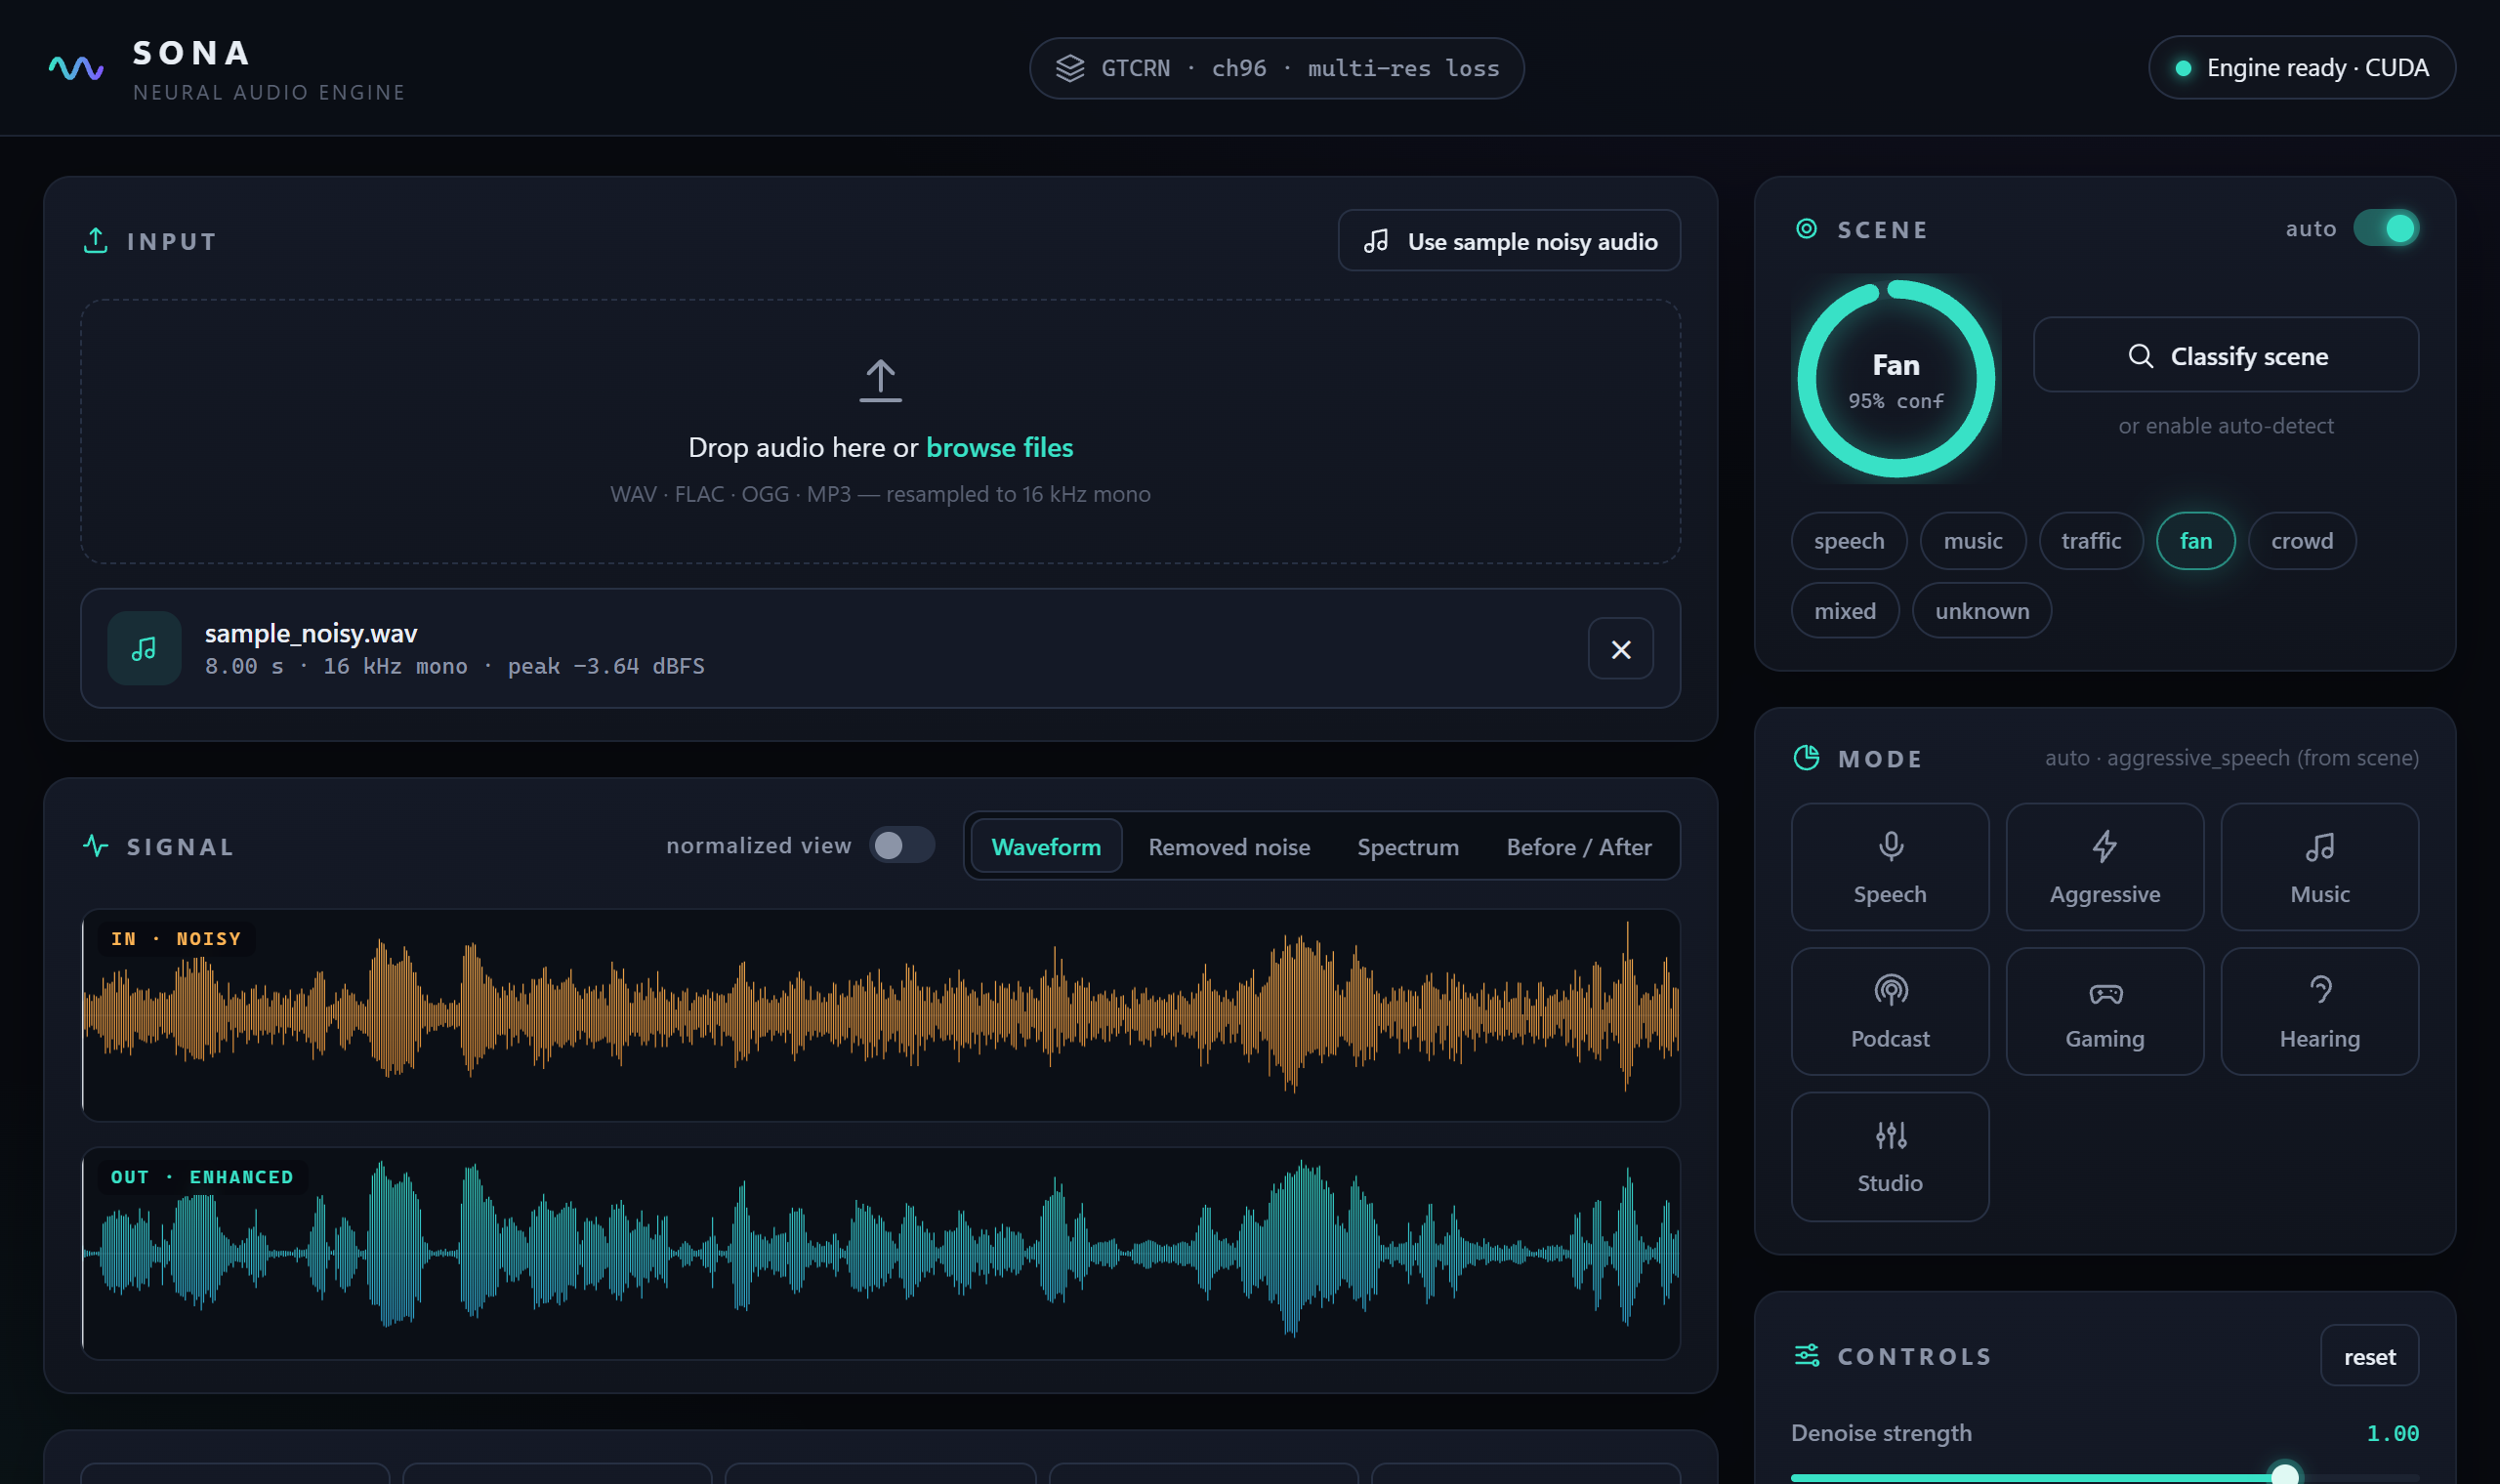
\includegraphics[width=\linewidth]{web_demo.png}
\caption{Real-time interactive system. The GTCRN engine (top bar) enhances the
loaded noisy signal; the noisy input (orange) and enhanced output (teal)
waveforms are shown, with automatic scene detection (right) routing the
suppression mode.}
\label{fig:web}
\end{figure}

%======================================================================
\section{Conclusion}
We showed that classical single-channel noise cancellation, though fast, is
unsuited to real non-stationary noise: on VoiceBank-DEMAND every classical
baseline degrades the signal (negative SI-SDRi) by stripping weak speech. A
compact, context-aware learned per-band filter---a 722\,K-parameter GTCRN on a
shared STFT front-end---reverses this, gaining $+9.9$~dB SI-SDRi, improving
intelligibility, and generalising to unseen noise, all at over 100$\times$ real
time. Ablations show that added architectural capacity does not help, that
complex masking trades perceptual score for waveform fidelity, and that guarded
test-time adaptation offers a small safe refinement. The novelty of this work is
methodological as much as architectural: a fair, shared-front-end comparison
that isolates the learned estimator, honest reporting including negative and
trade-off results, and a real-time edge-oriented system. Future work will
complete on-device deployment, a live microphone demonstration, and a
word-error-rate study, and will pursue perceptual-objective training to close
the PESQ gap to state-of-the-art.

%======================================================================
\begin{thebibliography}{99}
\bibitem{boll} Boll, S.: Suppression of acoustic noise in speech using spectral
subtraction. IEEE Trans. Acoust. Speech Signal Process. \textbf{27}(2),
113--120 (1979)
\bibitem{lim} Lim, J., Oppenheim, A.: Enhancement and bandwidth compression of
noisy speech. Proc. IEEE \textbf{67}(12), 1586--1604 (1979)
\bibitem{ephraim} Ephraim, Y., Malah, D.: Speech enhancement using a
minimum mean-square error short-time spectral amplitude estimator. IEEE Trans.
Acoust. Speech Signal Process. \textbf{32}(6), 1109--1121 (1984)
\bibitem{donoho} Donoho, D.: De-noising by soft-thresholding. IEEE Trans. Inf.
Theory \textbf{41}(3), 613--627 (1995)
\bibitem{rnnoise} Valin, J.-M.: A hybrid DSP/deep learning approach to real-time
full-band speech enhancement. In: IEEE MMSP (2018)
\bibitem{dccrn} Hu, Y., et al.: DCCRN: Deep complex convolution recurrent
network for phase-aware speech enhancement. In: Interspeech (2020)
\bibitem{deepfilternet} Schr\"oter, H., et al.: DeepFilterNet2: Towards
real-time speech enhancement on embedded devices. In: IWAENC (2022)
\bibitem{gtcrn} Rong, X., et al.: GTCRN: A speech enhancement model requiring
ultralow computational resources. In: IEEE ICASSP (2024)
\bibitem{metricgan} Fu, S.-W., et al.: MetricGAN+: An improved version of
MetricGAN for speech enhancement. In: Interspeech (2021)
\bibitem{squim} Kumar, A., et al.: TorchAudio-SQUIM: Reference-less speech
quality and intelligibility measures. In: IEEE ICASSP (2023)
\bibitem{voicebank} Valentini-Botinhao, C., et al.: Investigating RNN-based
speech enhancement methods for noise-robust text-to-speech. In: SSW (2016)
\bibitem{msnsd} Reddy, C.K.A., et al.: A scalable noisy speech dataset and
online subjective test framework (MS-SNSD). In: Interspeech (2019)
\bibitem{stoi} Taal, C.H., et al.: An algorithm for intelligibility prediction
of time-frequency weighted noisy speech. IEEE Trans. Audio Speech Lang. Process.
\textbf{19}(7), 2125--2136 (2011)
\bibitem{pesq} Rix, A.W., et al.: Perceptual evaluation of speech quality
(PESQ). In: IEEE ICASSP (2001)
\bibitem{sisdr} Le~Roux, J., et al.: SDR -- half-baked or well done?
In: IEEE ICASSP (2019)
\end{thebibliography}

\end{document}
